% Created 2020-06-21 Sun 16:58
% Intended LaTeX compiler: pdflatex
\documentclass[11pt]{article}
\usepackage[utf8]{inputenc}
\usepackage[T1]{fontenc}
\usepackage{graphicx}
\usepackage{grffile}
\usepackage{longtable}
\usepackage{wrapfig}
\usepackage{rotating}
\usepackage[normalem]{ulem}
\usepackage{amsmath}
\usepackage{textcomp}
\usepackage{amssymb}
\usepackage{capt-of}
\usepackage{hyperref}
\author{Jesus Rodolfo Izurieta Veliz}
\date{\today}
\title{Informe sesión de programación 2. Node Js}
\hypersetup{
 pdfauthor={Jesus Rodolfo Izurieta Veliz},
 pdftitle={Informe sesión de programación 2. Node Js},
 pdfkeywords={},
 pdfsubject={},
 pdfcreator={Emacs 26.3 (Org mode 9.4)}, 
 pdflang={English}}
\begin{document}

\maketitle
\tableofcontents

\pagebreak

\section{Introducción}
\label{sec:org09fb854}
\textbf{Enunciado del proyecto}

Desarrollo de un servidor web que atienda peticiones de archivos con diferentes formatos (ASCII, JSON, HTML, PDF).
Los archivos estarán distribuidos en dos únicos directorios: \emph{pub y /doc).
Cuando el servidor reciba una petición GET con la ruta ‘/doc}', deberá recuperarlo desde el directorio /doc;
el mismo procedimiento deberá seguirse con la ruta ‘/pub'. Por ejemplo: /pub/test.html

El servidor deberá verificar si el archivo solicitado existe antes de recuperarlo,
de lo contrario deberá retornar una página comunicando esta condición de error (Codigo 404 – Not Found).
Use los módulos “http”, “url” y “fs” de Node.

\section{Descripción}
\label{sec:org60b8877}
Para la creación del servidor con NodeJs, usaremos algunos módulos de npm,
entre ellos, url y fs; los instalamos con el manejador de módulos npm.

\subsection{Módulos importados}
\label{sec:org3fc123c}

\subsubsection{Url}
\label{sec:org803fb4d}
El módulo url de node, nos provee utilidades para la resolución de urls.
Para esto, cuenta con la clase url, lo que añade atributos que no serían accesibles en el caso de usar únicamente cadenas de texto.

\subsubsection{Fs}
\label{sec:org95ed0de}
El módulo fs implementa una interfaz del sistema de archivos del sistema operativo para node,
de modo que con ayuda de fs seremos capaces de acceder a directorios y archivos de nuestro servidor.

\section{Desarrollo}
\label{sec:org11739bc}

\subsection{Servidor http}
\label{sec:org3f0dd20}
Creamos el archivo app.js, donde pondremos el código del servidor,
lo primero que incluiremos en el documento serán los módulos importados que usaremos:

\begin{verbatim}
const http = require('http');
const url  = require('url');
const fs   = require('fs');
const path = require('path');
\end{verbatim}

Http es el módulo que nos permitirá recibir y responder a peticiones http.
Url contiene utilidades para resolución de urls.
Fs nos dará acceso al sistema de archivos del sistema operativo.
Path nos provee utilidades para el correcto manejo de direcciones de archivos.

A continuación definimos algunas variables para configurar el servidor:

\begin{verbatim}
const serverHostname  = 'http://localhost:8080/';
const serverPort = 8080;
\end{verbatim}

Nos servirán para definir el nombre del host y el número de puerto de nuestro servidor web.
Seguidamente desarrollamos el servidor, donde aceptaremos las peticiones usando el módulo http.

\begin{verbatim}
http.createServer()
\end{verbatim}

La función createServer del módulo http recibe una función con dos parámetros,
dos objetos: request y response que contienen la información de la petición
y proveen un medio para enviar una respuesta, respecticamente.
Esta función nos devolverá un objeto del que podremos llamar a su método listen con el puerto y el nombre del host,
para que el servidor escuche peticiones.

\begin{verbatim}
http.createServer(/* código del servidor */)
    .listen(serverPort, serverHostname);
\end{verbatim}

\subsection{Respuesta a peticiones de archivos}
\label{sec:org401bc76}
La función que pasaremos como parámetro de http.createServer contendrá el código
para responder a las peticiones realizadas por un cliente como un navegador.

\begin{verbatim}
function server (req, res) { /* código de servidor */ }
\end{verbatim}

Primeramente obtendremos la url y la convertiremos en un objeto de tipo URL,
para poder usar los métodos que implementa esta clase.
Creamos una nueva instancia de la clase URL, a la que pasamos como parámetros la url obtenida por la petición
y el nombre del host del servidor, variable que instanciamos anteriormente.

\begin{verbatim}
let request_url = new URL(req.url, serverHostname);
\end{verbatim}

Usaremos el método join de la clase path, para obtener la dirección local,
concatenando el directorio actual ('.') y la dirección del archivo que devolveremos,
que corresponde a la dirección de la url de la petición,
valor que podremos encontrar en el atributo pathname del objeto URL.

\begin{verbatim}
let filename = path.join('.', request_url.pathname);
\end{verbatim}

Finalmente, con el nombre y dirección del archivo al que se quiere acceder,
usamos el módulo fs para obtener el archivo (si existe),
Para esto usaremos el método readFile de fs, que recibe como parámetros el nombre del archivo,
el tipo de codificación, y un callback, una función que nos dará acceso a dos parámetros:
error, nos devolverá un error si no se puede obtener o abrir el archivo,
y data, que nos devolverá el contenido del archivo si este fue encontrado y pudo ser accedido sin problemas.

\begin{verbatim}
fs.readFile(filename, 'utf-8', function(err, data) {
    if(err){
        res.setHeader('Content-Type', 'application/json');
        res.statusCode = 404;
        let message = {
            code: "404: Not Found",
            message: "No se encuentra el archivo " + filename
        }
        res.end(JSON.stringify(message));
    }
    else {
        res.end(data);
    }
});
\end{verbatim}

En caso de que no haya errores en la lectura del archivo, el parámetro err será nulo,
por lo que preguntamos si es un valor definido en un if.
Si 'error' no es nulo, responderemos con un mensaje de error en formato json,
para esto, definimos la cabecera de la respuesta como 'application/json' y
el statusCode a 404

\begin{verbatim}
res.setHeader('Content-Type', 'application/json');
res.statusCode = 404;
let message = {
    code: "404: Not Found",
    message: "No se encuentra el archivo " + filename
}
res.end(JSON.stringify(message));
\end{verbatim}

A continuación creamos un objeto message que contendrá el código de error 404
y un mensaje en texto que será legible por la persona que acceda al servidor.
Enviaremos este mensaje como parámetro de la función end del objeto response,
no sin antes convertirlo en una cadena con la función stringify del módulo JSON.

Finalemnte en caso de que el objeto sea encontrado y pueda ser leído,
enviamos su contenido, almacenado en la variable data.

\section{Observaciones}
\label{sec:org052d339}
Se debe implementar algún mecanismo de seguridad en este servidor, ya que al responder a cualquier url en la petición,
cualquier archivo es accesible, incluyendo código fuente del servidor o cualquier otro archivo dentro
del mismo directorio.

\section{Pruebas}
\label{sec:org60cbfb6}
Usaremos un navegador para probar el servidor, incluiremos distintos formatos de archivos y directorios.

Creamos un archivo index.html en el directorio doc y realizando la petición \url{http://localhost:8080/doc/index.html} obtenemos:

\begin{center}
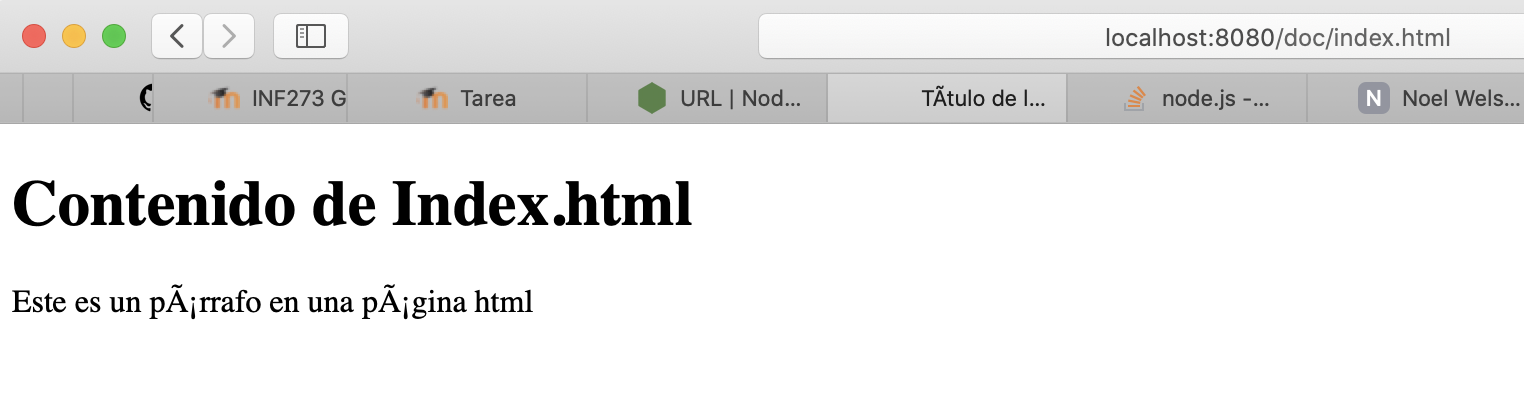
\includegraphics[width=.9\linewidth]{./captura.png}
\end{center}

De igual manera, con un archivo de texto, obtenemos el contenido de este:
\begin{center}
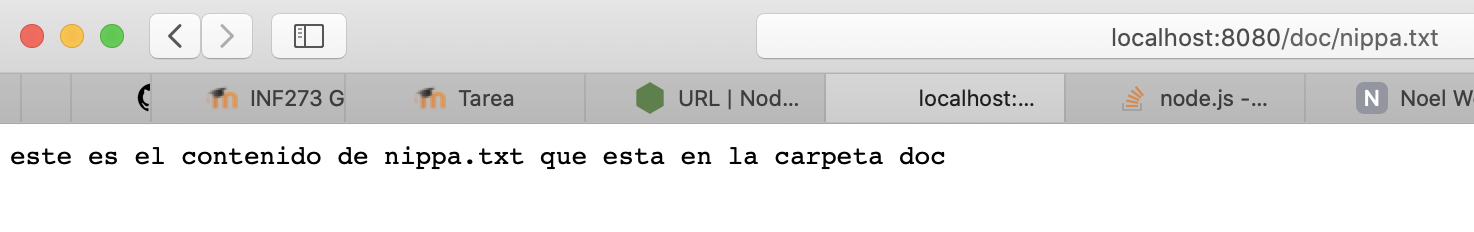
\includegraphics[width=.9\linewidth]{./captura2.png}
\end{center}
\end{document}
